\section{Component Selection}
\subsection{Transformer Selection}
According to design calculations and simulation results, Peak current of the transformer 10.8 Ampere, turn ratio of the transformer is 1.9:1, primary turn number of transformer 10, secondary turn number 5, Transformer primary side voltage is between 24-48 V which is input voltage range. To obtain required turn numbers, the cross-section area of the core must be smaller than 40 $mm^2$ and core saturation density of the available cores B=1 Tesla. According to the required cross-section area range, KOOL MU 2510 E core was chosen. Cross-section area of the chosen core is 38.5 $mm^2$. Permeability of the core is given in Figure \ref{fig:Permeability}. Permeability of the KOOL MU 2510 E Core is 90$\mu$. 

\begin{figure}[!h]
\centering
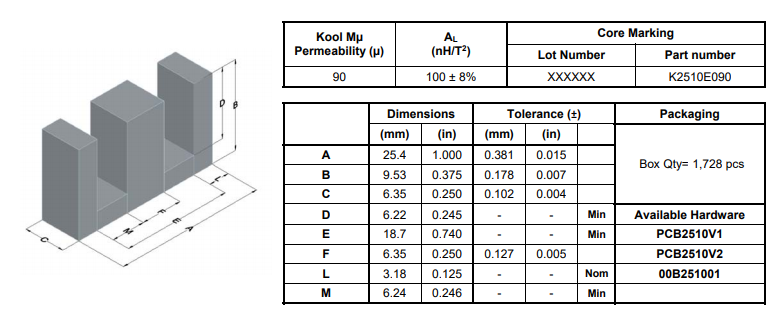
\includegraphics [width=1\textwidth]{core.png}
\caption{Detailed dimensions of the E core and relative permeability of core }
\label{fig:Permeability}
\end{figure}

The cross-section area is important to decide turn numbers and the gap between cores. Information about cross-section area and path length is given Figure \ref{fig:Csa}. As seen in (13), the gap is directly affected by path length and relative permeability, so both path length and relative permeability are also crucial for design.

\begin{align}
    gap=\frac{\mu_0\times N_P^2 \times A_e}{L_P}-\frac{l_e}{\mu_c}
\end{align}
Magnetic flux density of the core can be calculated by given formula;
\begin{align}
    B=\frac{\mu_0\times N_P\times A_e}{\frac{l_e}{\mu_c}+gap}
\end{align}

As seen from formula (14), magnetic flux density depends on the cross-sectional area, path length and relative permeability of the core. Cross-sectional area and relative permeability is limited since core can be saturated. Magnetic flux density is inversely proportional with gap and path length. As seen from Figure \ref{fig:SFD}, saturation flux density of the KOOL MU magnetic cores is 1 Tesla. Core shape, cross-section area and path length are chosen according to the saturation flux density of the KOOL MU magnetic core.

\begin{figure}[!h]
\centering
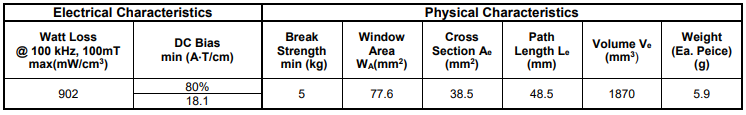
\includegraphics [width=1\textwidth]{area vs.png}
\caption{Cross section area and Path Length of core }
\label{fig:Csa}
\end{figure}
\begin{figure}[H]
\centering
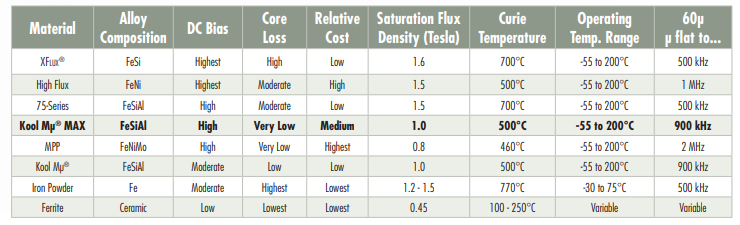
\includegraphics [width=1\textwidth]{permeability.png}
\caption{Saturation Flux Densities of various magnetic cores }
\label{fig:SFD}
\end{figure}
\subsection{Analog Controllers & Components}

Two analog controllers are used in the project for a highly flexible, efficient and feature-packed converter. The main controller is  UCC28740 Constant-Voltage Constant-Current Flyback Controller
Using Optocoupled Feedback by Texas Instruments. It will be powered by an auxiliary winding wound to the transformer. It is designated to be always used in DCM operation. It can take feedback from both primary and secondary sides and can keep output voltage constant and performs well in load and line regulation aspects. It has an embedded MOSFET driver to save space lower the component count. Furthermore, its internal algorithm also provides soft-switching to lower the initial stresses on the components.

To control synchronous switching in the secondary, UCC24636 Synchronous rectifier controller With Ultra-Low Standby current is used. It helps to replace the secondary side diode with a MOSFET to mimic its operation. As a result, the loss on diode is eliminated. Since losses on the MOSFET will be significantly lower, overall efficiency is improved. In Figure \ref{fig:refdesign2} a reference design which includes both controllers is given.

\begin{figure}[!h]
\centering
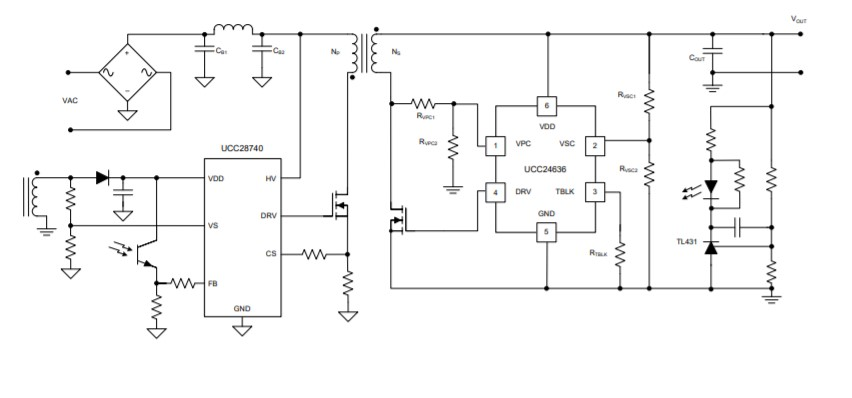
\includegraphics [width=0.6\textwidth]{refdesign2.jpg}
\caption{Flyback Controller Reference Design with UCC28749 and UCC24636}
\label{fig:refdesign2}
\end{figure}

\subsection{Cable Selection}
$\delta$= Skin Depth\\
$\rho$= Resistivity of Material\\
$\mu_r$= Relative Permeability of Cable\\
$\mu_0$= Permeability Constant = $4\pi\times 10^{-7}$
f= switching frequency = 45 kHz
\begin{align}
    \delta=\sqrt{\frac{\rho}{\pi\times f\times \mu_r\times \mu_0}}
\end{align}
Copper cable will be used in this flyback converter.
\begin{align}
\delta=\frac{7.5}{\sqrt{f}} cm   \\      \delta=\frac{7.5}{45000}=1.67\times 10^{-4} cm
\end{align}

At 45 kHz switching frequency, skin depth of copper cable is 1.67\times $10^{-4}$ cm. There is maximum 3 Ampere average current on transformer cable, so diameter of the cable must carry 3 ampere average current. To carry 3 ampere, AWG of the cable must be lower than #25 AWG. To avoid unexpected damages to our circuit, #20 AWG copper cable will be used.

\subsection{MOSFET Selection}
For the MOSFET selection, we need to consider the maximum voltage and current stresses over the MOSFET.

The maximum voltage stress over the MOSFET is obtained analytically by the following relation.

$$ V_{sw,peak} = V_{in,max} + \frac{N_P}{N_S}V_{out} $$

where $ V_{in,max} = 48\;V $, $ V_{out} = 15\;V $ and $ \frac{N_P}{N_S} = 1.9 $.

Then, the peak voltage over the MOSFET is computed analytically as follows:

$$ V_{sw,peak} = 48 + 1.9*15 = 76.5\;V $$

This value is in parallel with the peak voltage value obtained from the simulations of the Flyback Converter circuit in Simulink.

The peak voltage value for the MOSFET is obtained as $ V_{sw,peak} = 76.63 V $ from simulations.

The maximum current stress over the MOSFET is obtained analytically by the following relation.

$$ I_{sw,peak} = \frac{1}{(1-D)}\frac{N_S}{N_P}I_o + \frac{N_P}{N_S}\frac{(1-D)T_s}{2L_m}V_o $$

where $ I_o = \frac{P_o}{V_o} = \frac{60}{15} = 4\;A $

Then, the peak MOSFET current is found as follows:

$$ I_{sw,peak} = \frac{1}{(1-0.26)}*\frac{1}{1.9}*4 + 1.9*\frac{(1-0.26)*(1/45000)}{2*28.67*10^{-6}}*15 = 11\;A$$

One thing to notice here is that this peak current is computed assuming CCM operation. However, in our design, the converter mostly operates in DCM as seen from the voltage and current figures presented in the Simulation Results part. Therefore, for the MOSFET peak current value, we need to rely on the simulation results.

From the simulations of the Flyback Converter circuit in Simulink, the MOSFET peak current is observed as $ I_{sw,peak} = 9.690\;A $

Overall, the peak voltage and current ratings for the MOSFET is found as follows:

$$ V_{sw,peak} = 76.63\;V $$
$$ I_{sw,peak} = 9.690\;A $$
$$ I_{sw,mean} = \frac{I_{out}}{N_{PS}} = 2.1A $$

The selected MOSFET should also be able to handle the switching frequencies as high as 45 kHz. 
Since it is a very commonly used value, choosing a 100v MOSFET is reasonable. AOD482 by Alpha-Omega is a good choice since it is rated at 5A continuous, has a low ON resistance and costs relatively low.

\subsection{Diode Selection}
Similar to the MOSFET selection, the maximum voltage and current stresses over the diode must be determined for the diode selection.

The maximum reverse voltage across the diode during its off period can be calculated as
\begin{align*}
    V_D=V_{out}+N_{PS}V_{in,max}=-40.26V
\end{align*}
It is observed to be $ V_{diode,peak} = -40.26\;V $ from the simulations.

The maximum forward current through the diode during its on period can be calculated as:
\begin{align*}
    I_{s,peak}=\frac{2P_{out}}{D_{MAG}V_{OUT}}=18.89A
\end{align*} It is observed to be $ I_{diode,peak} = I_{s,peak} = 18.34\;A $ from the simulations.

Overall, the peak voltage and current ratings for the diode is found as follows:

$$ V_{diode,peak} = -40.26\;V $$
$$ I_{diode,peak} = 18.34\;A $$

Also, it should be noted that the average current of the diode will be equal to the output. Therefore SS5P5 from Vishay is chosen which is a Fast Recovery Schottky diode with 50V and 5A continuous rated diode which is right for the job.

\subsection{Output Capacitor Selection}
The average voltage across the output capacitor is equal to the average output voltage.

$$ V_{cap,avg} = V_{out} = 15\; $$

Then, the rated voltage of the selected capacitor must be greater than 15 V.

$$ V_{cap,rated} > 15\;V $$

One another limitation on the capacitor selection is the peak-to-peak output voltage ripple limit of the project. The peak-to-peak output voltage ripple is required to be less than 4\%.

$$ \frac{\Delta V_o }{V_o} = 0.04\;(4\%) $$

Then, the maximum allowable output voltage ripple is found as:

$$ \Delta V_o = 0.04*15\;V = 0.6\;V $$ 

Also, let's calculate the maximum allowable ESR for the required ripple.
\begin{align*}
    ESR_{C_{OUT}}=\frac{0.9V_ripple}{I_{s,max}}=20m\Omega
\end{align*}
The output voltage ripple for the Flyback Converter topology is computed from the following relation.

$$ \frac{\Delta V_o }{V_o} = \frac{DT_s}{RC} = \frac{D}{RCf_s} $$

Then, the minimum required output capacitance value is obtained as follows:

$$ C_{min} = \frac{D}{0.04*R*f_s} $$

where $ R = \frac{V_o^2}{P_o} = \frac{15^2}{60} = \frac{225}{60} = 3.75\;\ohm $

$$ C_{min} = \frac{0.26}{0.04*3.75*45000} = 77.8\;\micro F $$

Also, let's calculate the maximum allowable ESR for the required ripple.

\begin{align*}
    ESR_{C_{OUT}}=\frac{0.9V_ripple}{I_{s,max}}=20m\Omega
\end{align*}

Since it is either hard to find or very costly, using ceramic capacitors can not be used. Instead, using electrolytic capacitors in series is a good idea. However, we need to use them in parallel to reduce the ripple. Moreover, since ESR generally increases with lower capacitance a good balance needs to be found.

Using two of ESY477M025AG6AA capacitors from KEMET is a good solution. Since they have an ESR of 0.41m$\Omega$ and 470$\mu$F capacitance, they satisfy the ripple requirement.
From the simulations of the converter circuit in Simulink with the chosen output capacitor, the output voltage ripple is observed to be approximately 0.36 V, which is much lower than the maximum allowable output voltage ripple value of 0.6 V, as computed above.

The peak to peak current ripple on the output capacitor is also obtained from simulations of the converter circuit in Simulink with the chosen capacitors used. The peak to peak current ripple on the output capacitor is observed to be approximately 18.16 A.